%!TEX root = geometry.tex
\stepcounter{lecture}
\setcounter{lecture}{6}
\sektion{Geodesics}

\newcommand{\tgamma}{\tilde{\gamma}}

Let $g$ be a Riemannian metric on some open set $U\subset \R^2$, say
\begin{equation*}
	g = E \dif{x^2} + 2F \dif{x} \dif{y} + G \dif{y^2}.
\end{equation*}
The basis problem we want to answer is: given $p,q\in U$, how can we find the shortest path with respect to $g$ from $p$ to $q$, supposing it exists? These shortest paths are the analogues of lines in hyperbolic space.

\subsection{Energy functionals} % (fold)
\label{sub:energy_functionals}

Let $\gamma:[0,1] \to U$ be a smooth path. As we've seen before the length is
\begin{equation*}
	L_g(\gamma) = \int_0^1 \left.|\gamma\p(t)|\right._g \dif{t}.
\end{equation*}
This is invariant under reparameterisation:
\begin{equation*}
	L_g(\gamma\circ f) = L_g(\gamma),
\end{equation*}
where $f:[0,1] \to [0,1]$ is monotone and continuous.

Now we introduce a new function, which is not invariant under reparameterisation. This might seem like a bad thing, but actually it makes our lives a lot easier.

\begin{definition}
	The \emph{energy} of a smooth path $\gamma:[0,1] \to U$ is
	\begin{equation*}
		E_g(\gamma) = \int_0^1 \left.|\gamma\p(t)|\right._g^2 \dif{t}.
	\end{equation*}
\end{definition}

Recall the Cauchy-Schwarz inequality, which we've met in many different contexts:
\begin{equation*}
	\textstyle \int ab \leq \sqrt{\int a^2} \, \cdot \sqrt{\int b^2},
\end{equation*}
with equality if and only if $a=\lambda b$ or $b=\lambda a$, for some $\lambda$. Then
\begin{equation*}
	L_g(\gamma)
	= \int_0^1 \left.|\gamma\p(t)|\right._g \dif{t}
	\leq \sqrt{\int_0^1 \left.|\gamma\p(t)|\right._g^2 \dif{t}} \, \cdot \sqrt{\int_0^1 \dif{t}}
	= \sqrt{E_g(\gamma)},
\end{equation*}
with equality if and only if $\left.|\gamma_p(t)|\right._g = \lambda \cdot 1$ (a constant function); that is, if $\gamma$ has constant speed. Now, every $\gamma$ with $\gamma\p(t) \neq 0$ for all $t$ has a constant speed reparametrisation; consider
\begin{equation*}
	\tgamma = \gamma \circ f, \qquad
	f:[0,1] \to [0,1], \qquad
	f(s) = F^{-1}(s),
\end{equation*}
where $F:[0,1] \to [0,1]$ is given by 
\begin{equation*}
	F(s) = \f{\int_0^s \left.|\gamma_p(t)|\right._g \dif{t}}{\int_0^1 \left.|\gamma_p(t)|\right._g \dif{t}}.
\end{equation*}

\begin{definition}
	If $p,q \in U$, then the set of paths from $p$ to $q$ is given by $\Omega_{p,q}$; formally,
	\begin{equation*}
		\Omega_{p,q} = \left\{\text{$\gamma:[0,1]\to U$ smooth}: \gamma(0)=p, \gamma(1)=q\right\}.
	\end{equation*}
\end{definition}

\begin{proposition}
	The following two conditions are equivalent:
	\begin{enumerate}
	    \shortskip
		\item $E(\gamma_0) \leq E(\gamma)$ for all $\gamma\in\Omega_{p,q}$;
		\item $L(\gamma_0) \leq L(\gamma)$ for all $\gamma\in \Omega_{p,q}$, and $\gamma$ has constant speed.
	\end{enumerate}
\end{proposition}

\begin{proof}
	(i) $\implies$ (ii). If $\tgamma_0$ has constant then, then
	\begin{equation*}
		E(\tgamma_0)
		= \left[ L(\tgamma_0) \right]^2
		= \left[ L(\gamma_0) \right]^2
		\leq E(\gamma_0),
	\end{equation*}
	with equality if and only if $\gamma_0$ has constant speed; that is, $\gamma_0 = \tgamma_0$.

	(ii) $\implies$ (i). We have
	\begin{equation*}
		E(\gamma_0)
		= \left[ L(\gamma_0) \right]^2
		\leq \left[ L(\tgamma_0) \right]^2
		\leq E(\gamma),
	\end{equation*}
	which is what we require.
\end{proof}

\vspace{3pt}

\begin{note}
	If $\gamma\p(a) = 0$ for some $a\in[0,1]$, then can always find $F$ such that $E(\gamma \circ f) < E(\gamma)$.
\end{note}

% subsection energy_functionals (end)

\subsection{Calculus of variations} % (fold)
\label{sub:calculus_of_variations}

Given $H=H(x,y,z,w)$, suppose $\gamma\in\Omega_{p,q}$ minimises
\begin{equation*}
	\Phi(y) = \int_0^1 H(\gamma_1(t), \gamma_2(t), \gamma\p_1(t), \gamma\p_2(t)) \dif{t}
\end{equation*}
if, for example,
\begin{equation*}
	H(x,y,z,w) = E(x,y)\,z^2 + 2F(x,y) \, zw + G(x,y)\,w^2.
\end{equation*}
Then $\Phi(\gamma) = E_g(\gamma)$.

For any $\delta:[0,1] \to \R^2$ with $\delta(0)=\delta(1)=0$, if
\begin{equation*}
	(\gamma+\epsilon\delta)(t) = \gamma(t) + \epsilon\,\delta,
\end{equation*}
then $\gamma+\epsilon\delta \in \Omega_{p,q}$, when $\epsilon\ll1$. Thus $\epsilon=0$ minimises $\Phi(\gamma+\epsilon\delta)$:
\begin{align}
	0
	&= \dod{}{\epsilon}\Phi(\gamma+\epsilon\delta) \notag \\
	&= \int_0^1 \dod{}{\epsilon}\left[ (H(\gamma_1+\epsilon\delta_1, \gamma_2+\epsilon\delta_2, \gamma_1\p + \epsilon\delta_1\p, \gamma_2\p+\epsilon\delta_2\p) \right] \dif{t} \notag \\
	&= \int_0^1 \left[ H_x \delta_1 + H_y \delta_2 + H_z \delta_1\p + H_w \delta_2\p \right] \dif{t}. \label{eq:calc-variations}
\end{align}
Now we have
\begin{equation*}
	\int_0^1 H_z \delta_1\p \dif{t}
	= \left[ H_z \delta_1 \right]_0^1 - \int_0^1 \od{}{t}(H_z) \,\delta_1 \dif{t}
	= -\int_0^1 \od{}{t}(H_z)\,\delta_1 \dif{t},
\end{equation*}
as $\delta$ is a closed curve.

Returning to~\eqref{eq:calc-variations}, we see that
\begin{equation*}
	\int_0^1 \left[ \left( H_x - \dod{H_z}{t} \right)\delta_1 + \left( H_y - \dod{H_w}{t} \right)\delta_2 \right] \dif{t}
	\equiv 0,
\end{equation*}
for any $\delta_1,\delta_2$ with $\delta_i(0)=\delta_i(1) = 0$, $i=1,2$.

This gives us the \emph{Euler-Lagrange equations}:
\begin{equation*}
	H_x=\od{H_z}{t} \qqand
	H_y = \od{H_w}{t}.
\end{equation*}

% subsection calculus_of_variations (end)

\subsection{Geodesic equations} % (fold)
\label{sub:geodesic_equations}

\newcommand{\dgamma}{\dot{\gamma}}

In our case, we have
\begin{equation*}
	H(x,y,z,w) = E(x,y) \, z^2 + 2F(x,y)\,zw + G(x,y)\,w^2.
\end{equation*}
Simple differentiation gives us
\begin{equation*}
	H_x = E_x\,z^2 + 2F_x\,zw + G_x\,w^2 \qqand
	H_z = 2Ez + 2Fw.
\end{equation*}
Now we write $E(x,y) = E(\gamma_1(t), \gamma_2(t))$, and similar for $F$ and $G$. Letting a dot denote differentiation with respect to $t$, and substituting into the Euler-Lagrange equations, we obtain the \emph{geodesic equations}
\begin{align*}
	E_x \dot{\gamma}_1^2 + 2F_x \dgamma_1 \dgamma_2 + G_x \dgamma_2^2 &= \dod{}{t}(2E\dgamma_1 + 2F\dgamma_2), \\
	E_y \dgamma_1^2 + 2 F_y \dgamma_1 \dgamma_2 + G_y \dgamma_2^2 &= \dod{}{t}(2F\dgamma_1 + 2G\dgamma_2).
\end{align*}
This is a (nasty!) system of second-order differential equations.

\begin{definition}
	A path $\gamma:[a,b]\to U$ is a \emph{geodesic} if it satisfies the geodesic equations, or if is a critical points for the energy functional.

	A shortest length, constant speed path is a geodesic.
\end{definition}

\begin{theorem}
	Given $\pp\in U$ and $\xx\iR^2$, there is a unique geodesic $\gamma:(-\epsilon,\epsilon)\to U$ with $\gamma(0)=\pp$, $\gamma\p(0)=\xx$.
\end{theorem}

\begin{proof}
	This is an immediate consequence of the existence and uniqueness of solutions for ordinary differential equations.
\end{proof}

% subsection geodesic_equations (end)

	\pagebreak

\subsection{Exponential map} % (fold)
\label{sub:exponential_map}

\lecturemarker{14}{6 Mar}
\newcommand{\gvt}{\gamma_{\vv_\theta}}
\newcommand{\dGamma}{\dot{\Gamma}}

For $\pp\in U$, $\vv\iR^2$, there's a unique geodesic $\gamma_\vv:(-\epsilon,\epsilon) \to U$ with $\gamma(0)=\pp$, $\gamma\p(0)=\vv$. So why can't we extend this over all of $\R$? There are lots of reasons. Consider, for example, $U=\R^2\backslash\{0\}$. There is not geodesic linking the points $-x$ and $x$, $x\iR$, since we cannot go through the point $0$.

\begin{lemma}
	$\gamma_\vv(\lambda t) = \gamma_{\lambda\vv}(t)$, $\lambda\iR$.
\end{lemma}

\begin{proof}
	If $\gamma(t)$ satisfies the geodesic equations, so does $\gamma(\lambda t)$ (Both sides get multiplied by $\lambda^2$.) So $\overline{\gamma}=\gamma(\lambda t)$ is a geodesic with $\overline{\gamma}(0) = \gamma(0) = \pp$, $\overline{\gamma}\p(0) = \lambda\,\overline{\gamma}\p(0) = \lambda\vv$, and this gives us $\overline{\gamma} = \gamma_{\lambda\vv}$.
\end{proof}

\begin{definition}
	The \emph{exponential map} $\exp_\pp:B_\epsilon(0) \to U$ is given by
	\begin{equation*}
		\exp_\pp(\vv) = \gamma_\vv(1)
	\end{equation*}
\end{definition}

Note $\exp_\pp(\lambda \vv) = \gamma_{\lambda\vv}(1) = \gamma_\vv(\lambda)$, so $\exp_\pp(\vv)$ is defined for $|\vv|$ small.

\begin{proposition}
	$\eval[0]{\dif{\,\exp_\pp}}_0 = I$.
\end{proposition}

\begin{proof}
	Working from the definition, we have:
	\begin{align*}
		\eval[0]{\dif{\,\exp_\pp}}_0
		&= \lim_{\epsilon\to 0} \f{\exp_p(\epsilon\ww)-\exp_p(0)}{\epsilon} \\
		&= \lim_{\epsilon\to 0} \f{\gamma_{\epsilon\ww}(1) - \gamma_0(1)}{\epsilon} \\
		&= \lim_{\epsilon\to 0} \f{\gamma_\ww(\epsilon) - \gamma_\ww(0)}{\epsilon} \\
		&= \gamma\p_\ww(0) = \ww. \qedhere
	\end{align*}
\end{proof}

\begin{corollary}
	There are open sets $V_1 \subset \R^2$, $V_2\subset U$ with $0\in V_1, \pp\in V_2$, such that $\exp_p:V_1 \to V_2$ is a diffeomorphism; that is, differentiable, bijective and the inverse is differentiable.
\end{corollary}

\begin{proof}
	This follows from the inverse function theorem, since $I$ is invertible. Equivalently, we cause $\exp_p$ to define a new set of coords on $V_2$.
\end{proof}

% subsection exponential_map (end)

\subsection{Geodesic polar coordinates} % (fold)
\label{sub:geodesic_polar_coordinates}

Pick $\vv_1,\vv_2$ orthogonal with respect to the Riemannian metric $g_\pp$. Then we define
\begin{equation*}
	\vv_\theta = \vv_1 \cos\theta + \vv_2 \sin\theta.
\end{equation*}
This allows us to define the map
\begin{equation*}
	\fullfunction{T}{[0,\epsilon)}{[0,2\pi) \times U}{(r,\theta)}{\exp_p(r\vv_\theta)}.
\end{equation*}
These define a set of \emph{geodesic polar coordinates}.

Let $\overline{g} = \overline{E} \dif{r^2} + 2\overline{F} \dif{r}\dif{\theta} + \overline{G} \dif{\theta^2}$ be the metric induced from $g$ using $T$; that is,
\begin{equation*}
	\overline{E} = g(T_r,T_r),
	\qquad \overline{F} = g(T_r,T_\theta),
	\qquad \overline{G} = (T_\theta,T_\theta).
\end{equation*}

\begin{example}
	 Consider the Euclidean metric $g = g^E = \dif{x^2} + \dif{y^2}$, with exponential map $T(r,\theta) = \exp_0(r\vv_\theta) = r\vv_\theta$. Then
	 \begin{align*}
	 	x = r\cos\theta, & \qquad \dif{x} = \dif{r} - r\sin\theta \dif{\theta}, \\
	 	y = r\sin\theta, & \qquad \dif{y} = \dif{r} + r\cos\theta \dif{\theta}.
	 \end{align*}
	 Thus we have
	 \begin{equation*}
	 	\overline{g} = \dif{x^2} + \dif{y^2} = \dif{r^2} + r^2 \dif{\theta^2}.
	 \end{equation*}
\end{example}

We consider a similar problem on the third examples sheet:

\begin{example}
	We consider the metric on the disc:
	\begin{equation*}
		g = g^D = \f{4\left( \dif{x^2}+\dif{y^2} \right)}{\left( 1-x^2-y^2 \right)^2}.
	\end{equation*}
	Then our map is given by $T(r,\theta) = 2\tanh^{-1} r \vv_\theta$, and the induced metric is
	\begin{equation*}
		\overline{g} = \dif{r^2} + \sinh^2 r \dif{\theta}^2.
	\end{equation*}
\end{example}

There's a common pattern in both of these examples:

\vspace{3pt}

\begin{proposition}
	Under the notation established thus far, we have $\overline{E}=1$, $\overline{F}=0$, $\overline{G} = r^2 \tilde{G}(r,\theta)$ where $\lim_{r\to 0} \tilde{G}(r,\theta) = 1$.
\end{proposition}

\begin{proof}
	First we need a lemma:

	\vspace{8pt}

	\begin{lemma}
		Geodesics have constant speed:
		\begin{equation*}
			\left.|\gamma\p_\vv(t)|\right._g = \left.|\gamma\p_\vv(0)|\right._g = \left.|\vv|\right._{g_0}.
		\end{equation*}
	\end{lemma}

	\vspace{-3pt}

	Proof of the lemma is on the examples sheet. Now we can prove the proposition, tackling each function in turn:
	\begin{enumerate}
		\item From our previous work, we have
		\begin{equation*}
			T_r = \pd{}{r}(\gamma_{\vv_\theta}(r)) = \gamma\p_{\vv_\theta}(r).
		\end{equation*}
		Using our lemma, we thus have
		\begin{equation*}
			\overline{E}
			= g(T_r,T_r)
			= g(\gamma\p_{\vv_\theta}, \gamma\p_{\vv_\theta})
			= g(\gamma\p_{\vv_\theta}(0), \gamma\p_{\vv_\theta}(0))
			= g_0(\vv_\theta, \vv_\theta)
			= 1.
		\end{equation*}

		\item First consider the energy functional
		\begin{equation*}
			E_g^{[0,r]}(\gamma_{\vv_\theta})
			= \int_0^r g(\gamma\p_{\vv_\theta}, \gamma\p_{\vv_\theta}) \dif{t}
			= \int_0^r 1 \dif{t}
			= r.
		\end{equation*}
		Thus we have
		\begin{equation*}
			0
			= \pd{}{\theta}\left[ E_g^{[0,r]}(\gamma_{\vv_\theta}) \right]
			= \pd{}{\epsilon}\left[ E_g^{[0,r]}(\gvt + \epsilon\delta) \right],
		\end{equation*}
		where $\delta(t) = \pd{}{\theta}(\gvt(t)) = T_\theta(t,\theta)$.

		From our derivativation of the geodesic equations, we know
		\begin{align}
			&\dpd{}{\epsilon}\left[ E_g^{[0,r]}(\gvt + \epsilon\delta) \right] \notag \\
			&\qquad= \underbrace{\left[ H_z \delta_1 \right]_0^r + \left[ H_w \delta_2 \right]_0^r}_{\eqref{eq:calc-variations}} + \int_0^r \left( H_x - \dod{H_z}{t} \right) \delta_1 + \left( H_y - \dod{H_w}{t} \right) \delta_2 \dif{t}.
			\label{eq:induced-metric-geodesic}
		\end{align}
		The integral cancels to zero, since $\gvt$ is a geodesic. Hence,~\eqref{eq:calc-variations} and~\eqref{eq:induced-metric-geodesic} give
		\begin{equation*}
			2 \left[ \left.(E\dgamma_1 + F\dgamma_2)\right.\delta_1 + \left.(F\dgamma_1 + G\dgamma_2)\right. \delta_2 \right]
			= 2g(\gvt\p, \delta) = 0.
		\end{equation*}
		But $2g(T_r,T_\theta) = 2g(\gvt\p,\delta)$, so $\overline{F}=0$.

		\item First we consider
		\begin{equation*}
			T_\theta(0,\theta) = \pd{}{\theta}(\gvt(0)) = \pd{\pp}{\theta} = \vec{0}
		\end{equation*}
		Then we have
		\begin{align*}
			\dpd{T}{r}(T_\theta)(0,\theta) = T_{\theta r}(0,\theta) = T_{r\theta}(0,\theta)
			&= \dpd{}{\theta}T_r(0,\theta) \\
			&= \dpd{}{\theta}(\gvt\p(0)) \\
			&= \dpd{}{\theta}(\vv_\theta) \\
			&= -\vv_1 \sin\theta + \vv_2 \cos\theta = \vv_\theta^\perp
		\end{align*}
		Unpacking this, we deduce that
		\begin{equation*}
			T_\theta(r,\theta) = r\vv(r,\theta),
		\end{equation*}
		where $\lim_{r\to 0} \vv(r,\theta) = \vv_\theta^\perp$. Now
		\begin{equation*}
			\overline{G} = g(T_\theta, T_\theta) = r^2 g(\vv,\vv) = r^2 \tilde{G}(r,\theta),
		\end{equation*}
		where
		\begin{equation*}
			\lim_{r\to 0} \tilde{G}(r,\theta) = \lim_{r \to 0} g(\vv,\vv) = \eval[0]{g}_0(\vv_\theta^\perp, \vv_\theta^\perp) = 1. \qedhere
		\end{equation*}
	\end{enumerate}
\end{proof}

% subsection geodesic_polar_coordinates (end)

\subsection{Local Gauss-Bonnet} % (fold)
\label{sub:local_gauss_bonnet}

First we set up an open set $U\subset \R^2$ with geodesic polar coordinates $g=\dif{r^2} + G\dif{\theta^2}$, as discussed in the previous section. Let $\triangle OBC$ be a geodesic triangle.

\begin{center}
	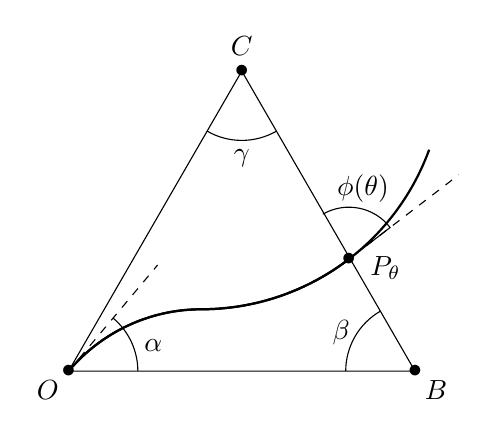
\begin{tikzpicture}[scale=2.2]
		\draw (0,0) node {$\bullet$} node [below left] {$O$}
		-- ++ (0:2) node {$\bullet$} node [below right] {$B$}
		-- ++ (120:2) node {$\bullet$} node [above=2pt] {$C$} -- cycle;

		\draw [thick] (0,0)
			arc (140:90:1)
			arc (270:307.5:1.4) node {$\bullet$} 
			arc (307.5:340:1.4);

		\draw [thick] (0,0)
			arc (140:90:1)
			arc (270:307.5:1.4) ++ (0,-0.05) node [right=4pt] {$P_\theta$};

		\draw [dashed] (0,0) -- ++ (50:0.8);
		\draw (0.4,0) arc (0:50:0.4);
		\draw (0.35,0.15) node [right=2pt] {$\alpha$};

		\draw (1.6,0) arc (180:120:0.4);
		\draw (2,0) ++ (120:1.6) arc (300:240:0.4);

		\draw (1,1.4) node [below=4pt] {$\gamma$};
		\draw (1.76,0.22) node [left=5pt] {$\beta$};

		\draw [dashed] (0,0) arc (140:90:1) arc (270:307.5:1.4) -- ++ (37.5:0.8);
		\draw (0,0) arc (140:90:1) arc (270:307.5:1.4) -- ++ (37.5:0.3) arc (37.5:120:0.3);

		\draw (1.7,0.92) node [above] {$\phi(\theta)$};
	\end{tikzpicture}
\end{center}

Geodesic triangles are formed by the arcs of three geodesics on a curved surface; straight lines are used above only for illustrative purposes. Here we have
\begin{align*}
	OB &= \left\{\theta=0, r\in[0,b]\right\}, \\
	OC &= \left\{\theta=\alpha, r\in[0,c]\right\}, \\
	BC &= \left\{\Gamma(\theta) = (f(\theta,\theta)), \theta\in[0,1]\right\}.
\end{align*}
Now let $P_\theta=\Gamma(\theta)$. Then $\phi(\theta)$ is the angle between $OP_\theta$ and $BC$. Note that $\phi(0) = \pi-\beta$ and $\phi(\alpha)=\gamma$.

The length of this curve $BP_\theta$, given by
\begin{equation*}
	s(\theta) = \int_0^\theta |\Gamma\p(u)| \dif{u}.
\end{equation*}
We then define
\begin{equation*}
	h(\theta) := \od{s}{\theta} = \left.|\Gamma\p(\theta)|\right._g
	\qquad
	\text{which gives us}
	\qquad
	\od{f}{s} = \od{f}{\theta} \od{\theta}{s} = \f{f\p(\theta)}{h(\theta)}.
\end{equation*}

\begin{lemma}
	$\disp \dod{}{s}\left( \f{f\p}{h} \right) = \f{G_r}{2h}.$
\end{lemma}

\begin{proof}
	If we parametrise by arc length $\Gamma$, then it satisfies the geodesic equations. Letting a dot denote differentiation with respect to $s$:
	\begin{equation*}
		\od{}{s}\left[ 2E\,\dGamma_1 + 2F\,\dGamma_2 \right] = E_r\,\dGamma_1^2 + F_r\,\dGamma_1 \, \dGamma_2 + G_r\,\dGamma_2^2.
	\end{equation*}
	Most terms didsppaear, leaving
	\begin{equation*}
		\od{}{s}\left( 2\dod{f}{s} \right) = G_r \left( \dod{\theta}{s} \right)^2.
	\end{equation*}
	Finally, this gives us
	\begin{equation*}
		2\,\od{}{s}\left( \f{f\p}{h} \right) = \f{G_r}{h^2},
	\end{equation*}
	which is easily rearranged to give the result.
\end{proof}

\begin{lemma}
	$\od{\phi}{\theta} \equiv \phi\p = (-\sqrt{G}\,)r.$
\end{lemma}

\begin{proof}
	In the diagram above, $OP_\theta$ is a ray of constant $\theta$, parameterised by $\rho(u) = (u,\theta)$ and $\rho\p(u) = (1,0)$. Now $\Gamma\p=(f\p,1)$, and then
	\begin{equation*}
		\cos \phi
		= \f{g(\Gamma\p, \rho)}{|\Gamma\p|_g |\rho\p|_g}
		= \f{f\p}{h \cdot 1}
		= \f{f\p}{h}. \tag{$*$}
	\end{equation*}
	Now we also consider
	\begin{equation*}
		\sin^2\phi
		= 1-\cos^2\phi
		= 1 - \left( \f{f\p}{h} \right)^2
		= 1-\f{(f\p)^2}{(f\p)^2 + G}
		= \f{G}{(f\p)^2 + G}
		= \f{G}{h^2}. \tag{$**$}
	\end{equation*}
	We thus have $\sin \phi = \sqrt{G}/h$. Then we differentiate $(*)$:
	\begin{equation*}
		-\phi\p \sin\phi = \left( \f{f\p}{h} \right)\p = \f{G_r}{2h},
	\end{equation*}
	by the previous lemma. Then
	\begin{equation*}
		\phi\p
		= -\f{G_r}{2h \sin\theta}
		= -\f{G_r}{2h} \left( \f{h}{\sqrt{G}} \right)
		= -\f{G_r}{2\sqrt{G}}
		= -(\sqrt{G}\,) r. \qedhere
	\end{equation*}
\end{proof}

This leads us to one of the main theorems of this chapter:

\begin{theorem}
	[Local Gauss-Bonnet theorem] For a geodesic triangle as described previously,
	\begin{equation*}
		\defect(OBC)
		= \alpha+\beta+\gamma-\pi
		= \iint_{OBC} \f{-(\sqrt{G}\,)_{rr}}{\sqrt{G}} \dif{A_g}.
	\end{equation*}
\end{theorem}

\begin{proof}
	We have $\dif{A_g} = \sqrt{\deg g} = \sqrt{G}$\,, so
	\begin{align*}
		\iint_{OBC} \f{(-\sqrt{G}\,)_{rr}}{\sqrt{G}} \dif{A_g}
		&= \int_0^\alpha \int_0^{f(\theta)} (-\sqrt{G}\,)_{rr} \dif{r} \dif{\theta} \\
		&= \int_0^\alpha \left[ -(\sqrt{G}\,)_r \right]_0^{f(\theta)} \dif{\theta} \\
		&= \int_0^\alpha \left[ (\sqrt{G}\,)_r \right]_{r=0} - \left[ (\sqrt{G}\,)_r \right]_{r=f(\theta)} \dif{\theta}.
		\intertext{Note $G=r^2 \tilde{G}$, with $\tilde{G} \to 1$ as $r\to 0$. Thus $\sqrt{G} = r \sqrt{\tilde{G}}$\,, and so $(\sqrt{G}\,)_r = \sqrt{\tilde{G}} + r(\sqrt{\tilde{G}}\,)_r \to 1$ as $r\to 0$. Then}
		&= \int_0^\alpha (1+\phi\p) \dif{\theta} \\
		&= \left[ \theta+\phi(\theta) \right]_0^\alpha \\
		&= \alpha+\gamma-\left( \pi-\beta \right) \\
		&= \alpha+\gamma+\beta-\pi. \qedhere 
	\end{align*}
\end{proof}

\begin{corollary}
	For $\triangle ABC \subset U$ with geodesic sides, we have
	\begin{equation*}
		\defect(ABC) = \iint_{\triangle ABC} \f{-(\sqrt{G}\,)_{rr}}{\sqrt{G}} \dif{A_g}.
	\end{equation*}
\end{corollary}

\begin{proof}[Sketch proof]
	Introduce a point $O$ as follows:
	
	\begin{minipage}{0.85\textwidth}
		\centering
		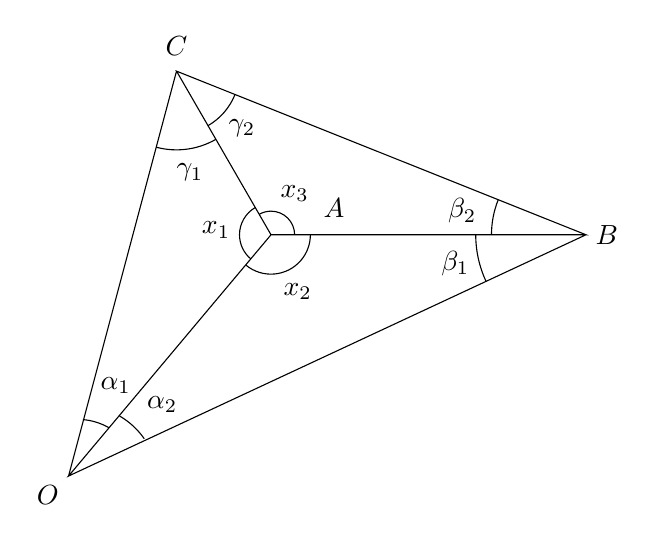
\begin{tikzpicture}[scale=2]

			\coordinate (A) at (0,0);
			\coordinate (B) at (2,0);
			\coordinate (C) at ++(120:1.2);
			\coordinate (O) at ++(230:2);

			\draw (A) -- (B) -- (C) -- (A) -- (O) -- (B) -- (C) -- (O);

			\draw (0.15,0) arc (0:120:0.15);
			\draw (0,0) ++ (120:0.2) arc (120:230:0.2);
			\draw (0,0) ++ (230:0.25) arc (230:360:0.25);

			\draw (B) ++ (-0.6,0) arc (180:158.217:0.6);
			\draw (B) ++ (-0.7,0) arc (180:205:0.7);

			\draw (B) ++ (169.1085:0.8) node {$\beta_2$};
			\draw (B) ++ (192.5:0.85) node {$\beta_1$};

			\draw (A) ++ (230:1.6) arc (60:85.06:0.4);
			\draw (A) ++ (230:1.5) arc (60:35:0.5);

			\draw (C) ++ (-21.79:0.4) arc (-21.79:-60:0.4);
			\draw (C) ++ (-60:0.5) arc (-60:-104.92:0.5);

			\draw (A) ++ (60:0.3) node {$x_3$};
			\draw (A) ++ (175:0.35) node {$x_1$};
			\draw (A) ++ (295:0.4) node {$x_2$};

			\draw (O) ++ (37.5:0.75) node {$\alpha_2$};
			\draw (O) ++ (62.525:0.65) node {$\alpha_1$};

			\draw (C) ++ (-40.895:0.55) node {$\gamma_2$};
			\draw (C) ++ (-82.475:0.65) node {$\gamma_1$};

			\draw (B) node [right] {$B$};
			\draw (A) ++ (0.4,0.05) node [above] {$A$};
			\draw (O) node [below left] {$O$};
			\draw (C) node [above=2pt] {$C$};
		\end{tikzpicture}
	\end{minipage}
	\begin{minipage}{0.13\textwidth}
		\begin{align*}
			\triangle_1 &= \triangle OAC \\
			\triangle_2 &= \triangle BAO \\
			\triangle_3 &= \triangle CAB
		\end{align*}
	\end{minipage}

	Let $\psi=\triangle_1 \cup \triangle_2 \cup \triangle_3$. Then
	\begin{align*}
		\defect(\triangle_1) + \defect(\triangle_2) + \defect(\triangle_3)
		&= \gamma_1 + \gamma_2 + \alpha_1 \alpha_2 + \beta_1 + \beta_2 + x_1 + x_2 + x_3 - 3\pi \\
		&= \gamma_1 + \gamma_2 + \alpha_1 \alpha_2 + \beta_1 + \beta_2 - \pi
		 = \defect(\triangle_4).
	\end{align*}
	We can apply local Gauss-Bonnet to $\triangle_1, \triangle_2, \triangle_4$:
	\begin{align*}
		\defect(\triangle_3)
		&= \defect(\triangle_4)-\defect(\triangle_1)-\defect(\triangle_2) \\
		&= \iint_{\triangle_4} (-1)\dif{A_g} - \iint_{\triangle_1} (-1) \dif{A_g} - \iint_{\triangle_2} (-1)\dif{A_g} \\
		&= \iint_{\triangle_3} \f{-(\sqrt{G}\,)_{rr}}{\sqrt{G}} \dif{A_g},
	\end{align*}
	as required. This is only a sketch proof because we need to consider different configurations of points and triangles, but the other cases are very similar.
\end{proof}

\begin{corollary}
	\begin{equation*}
		\lim_{A,B,C\to p} \f{\defect(ABC)}{\Area(ABC)} = \eval[-1]{-\f{(\sqrt{G}\,)_{rr}}{\sqrt{G}}}_p.
	\end{equation*}
\end{corollary}

\begin{definition}
	If $g$ is a Riemannian metric on $U$, then the \emph{Gauss curvature} at $p$ is given by
	\begin{equation*}
		K_p(g) := \lim_{A,B,C\to p} \f{\defect(ABC)}{\Area(ABC)}.
	\end{equation*}
\end{definition}

Now, isometries preserve angles and areas, so if $\phi:(U_1,g_1) \to (U_2,g_2)$, then $K_p(g_1) = K_{\phi(p)}(g_2)$. The corollary shows that the limit in the definition exists (which is the hard part to prove), and is given by
\begin{equation*}
	-(\sqrt{G}\,)_{rr}/\sqrt{G} \qquad \text{if} \qquad g=\dif{r^2} + G\dif{\theta^2}.
\end{equation*}

\begin{example}
	Consider $g=g^D$, the hyperbolic metric on $D$.  In geodesic polar coordinates, this is equivalent to
	\begin{equation*}
		\overline{g} = \dif{r^2} + \sinh^2 r \dif{\theta} \qqand
		\sqrt{G} = \sinh r,
	\end{equation*}
	and the curvature is given by
	\begin{equation*}
		K = -\f{(\sqrt{G}\,)_{rr}}{\sqrt{G}} = -\f{\sinh r}{\sinh 1} \equiv -1.
	\end{equation*}
\end{example}

\begin{corollary}
	If $ABC$ is a triangle in $\HH$, then $\defect(ABC) = -\Area(ABC)$.
\end{corollary}

% subsection local_gauss_bonnet (end)